\begin{cuzchapter}{系统概要设计}{chap:design}
    \usetikzlibrary{calc}

    %---------------------------------------------------------------------------%
    %->> 系统设计与实现章节写作指南
    %---------------------------------------------------------------------------%
    % 本章主要介绍本平台的设计思路、架构和实现方法
    % 一个完整的系统设计与实现章节应包含以下几个部分：
    % 1. 设计目标：明确系统的设计目标和原则
    % 2. 系统架构：介绍系统的整体架构和各组件的功能
    % 3. 关键技术：详细说明系统实现中使用的关键技术
    % 4. 实现细节：介绍系统的具体实现方法和过程
    % 5. 测试与评估：说明系统的测试方法和评估结果


    \section{系统功能结构设计}
    智能幻灯片协作平台，主要是为了为用户能够方便、高效地创作幻灯片而设计的，
    经过系统需求分析后，
    可以确定本平台主要实现用户登录、幻灯片管理、幻灯片评论、协作者权限管理、幻灯片创作、代码片段管理等功能模块。
    系统功能结构图如图\ref{fig:system-function-structure}所示。
    % 而这些功能模块中，幻灯片创作模块是最为核心的，尽可能满足用户在创作幻灯片时的各种需求，
    % 在协作编辑幻灯片文档前，用户通过协作者权限管理模块来管理协作者的权限，
    % 同时可以代码片段管理模块管理自定义的代码片段。
    % 最后通过在幻灯片管理模块以幻灯片空间的方式更方便地管理幻灯片，
    % 同时通过幻灯片评论来提供一定的反馈和交流，帮助用户进一步提升幻灯片的质量。
    

    \begin{figure}[htpb]
        \centering
        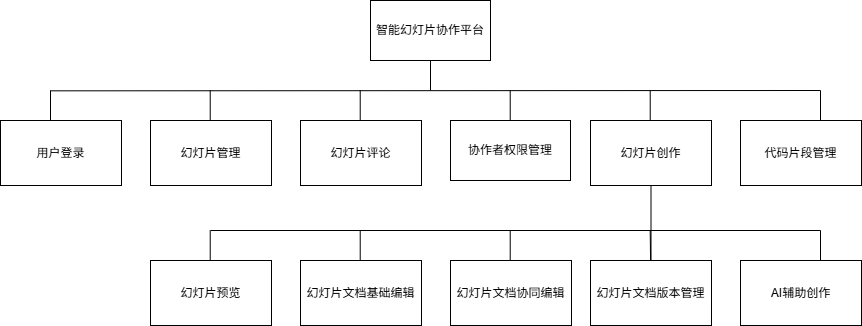
\includegraphics[width=0.9\textwidth]{figures/drawio/系统功能结构图-v2.drawio.png}
        \caption{系统功能结构图}
        \label{fig:system-function-structure}
    \end{figure}

    % \section{设计目标}\label{sec:design-goals}

    % % \subsection{设计目标}
    % % 作者希望开发一个简单易用的智能幻灯片协作平台，包括实时协作、权限管理、AI辅助、版本管理等核心功能。

    % % 本平台的设计目标如下：
    % % 支持多用户实时协作编辑，编辑过程中光标位置能够实时追踪。
    % % 权限控制基于RBAC模型，划分四级权限来管理文档访问。
    % % AI辅助生成幻灯片内容，同时提供兼容Slidev语法的建议。
    % % 版本管理方面，实现历史版本查看、差异对比和回滚操作。

    % 作者希望开发一个功能完善、简单易上手的智能幻灯片协作平台，主要实现以下目标：
    % 实时协作：当多个用户实时协作编辑时，可以让光标实时追踪；
    % 权限管理：基于RBAC模型设计四级权限，实现文档访问控制；
    % AI辅助功能：用AI辅助演讲者生成幻灯片，并提供合适于Slidev语法的智能建议；
    % 简单的版本管理：提供版本历史查看、差异对比和历史回滚等功能；

    % \subsection{设计原则}

    % 系统设计将遵循模块化设计、前后端分离等原则。

    % 在系统设计过程中，遵循以下设计原则：
    % 模块化设计：设计独立的功能模块，以便于维护和扩展；
    % 前后端分离：提高系统的灵活性和可维护性；
    % 简单易上手：用直观的用户界面减少非技术用户的学习成本；

    % \section{系统技术总体架构}\label{sec:system-architecture}

    % 本平台采用了前后端分离的架构。整体架构如图\ref{fig:appt-architecture}所示，包含前端展示层、后端业务层和数据存储层。
    % \begin{figure}[htbp]
    %     \centering
    %     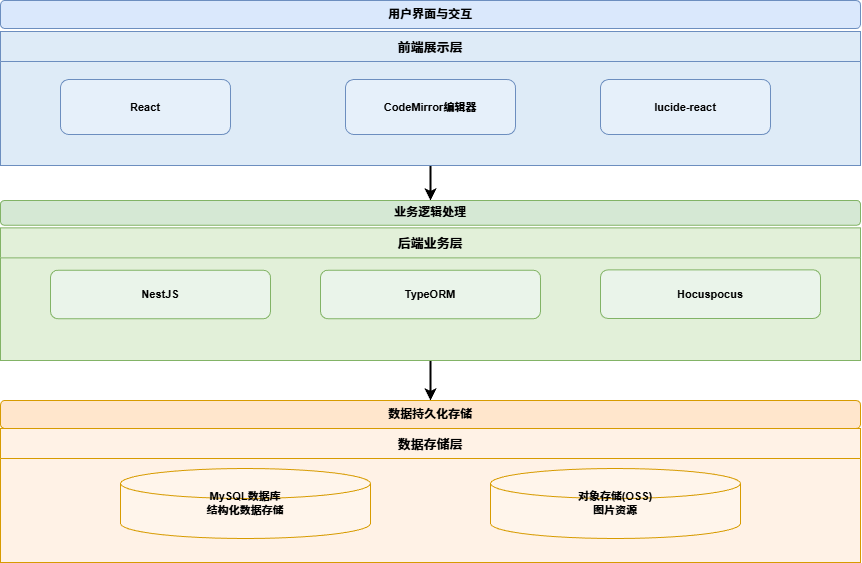
\includegraphics[width=0.9\textwidth]{figures/drawio/智能幻灯片协作平台整体架构图.drawio.png}
    %     \caption{系统技术总体架构}
    %     \label{fig:appt-architecture}
    % \end{figure}

    % % \begin{figure}[htbp]
    % %     \centering
    % %     \begin{tikzpicture}[
    % %             node distance=2cm and 3cm,
    % %             layer/.style={rectangle, draw, rounded corners, fill=white, align=center, minimum width=4cm, minimum height=1.2cm},
    % %             component/.style={rectangle, draw, fill=white, align=center, minimum width=3.5cm, minimum height=1.2cm},
    % %             arrow/.style={->, >=stealth, thick},
    % %             label/.style={text width=4cm, align=center, font=\small}
    % %         ]

    % %         \begin{scope}
    % %             % 定义层节点
    % %             \node[layer, fill=blue!10] (frontend) {前端展示层};
    % %             \node[layer, fill=green!10, below=3.5cm of frontend] (backend) {后端业务层};
    % %             \node[layer, fill=orange!10, below=3.5cm of backend] (storage) {数据存储层};

    % %             % 前端组件
    % %             \node[component, fill=blue!5, left=2.5cm of frontend] (react) {React应用};
    % %             % \node[component, fill=blue!5, left=2.5cm of frontend] (react) {React应用\\React 19 + TypeScript + Vite};
    % %             \node[component, fill=blue!5, right=2.5cm of frontend] (editor) {CodeMirror编辑器};
    % %             % \node[component, fill=blue!5, right=2.5cm of frontend] (editor) {CodeMirror 6编辑器\\Markdown语法高亮};
    % %             \node[component, fill=blue!5, above=1.5cm of react] (yjs) {Yjs客户端\\实时协作};
    % %             \node[component, fill=blue!5, above=1.5cm of editor] (slidev) {Slidev预览组件\\实时预览};

    % %             % 后端组件
    % %             \node[component, fill=green!5, left=2.5cm of backend] (nest) {NestJS框架\\RESTful API};
    % %             \node[component, fill=green!5, right=2.5cm of backend] (hocus) {Hocuspocus服务器\\WebSocket协作};
    % %             % \node[component, fill=green!5, above=1.5cm of nest] (business) {业务模块\\用户/幻灯片/权限管理};
    % %             \node[component, fill=green!5, above=1.5cm of hocus] (auth) {认证授权\\JWT + RBAC};

    % %             % 存储组件
    % %             \node[component, fill=orange!5, left=2cm of storage] (mysql) {MySQL数据库\\结构化数据存储};
    % %             \node[component, fill=orange!5, right=2cm of storage] (oss) {对象存储(OSS)\\图片与静态资源};

    % %             % 连接线
    % %             \draw[arrow] (react) -- (frontend);
    % %             \draw[arrow] (editor) -- (frontend);
    % %             \draw[arrow] (yjs) -- (frontend);
    % %             \draw[arrow] (slidev) -- (frontend);

    % %             \draw[arrow] (frontend) -- node[right] {HTTP/WebSocket} (backend);

    % %             \draw[arrow] (nest) -- (backend);
    % %             \draw[arrow] (hocus) -- (backend);
    % %             % \draw[arrow] (business) -- (backend);
    % %             \draw[arrow] (auth) -- (backend);

    % %             \draw[arrow] (backend) -- node[right] {数据持久化} (storage);

    % %             \draw[arrow] (mysql) -- (storage);
    % %             \draw[arrow] (oss) -- (storage);

    % %             % 标签
    % %             \node[label, above=0.5cm of frontend] {用户界面与交互};
    % %             \node[label, above=0.5cm of backend] {业务逻辑处理};
    % %             \node[label, above=0.5cm of storage] {数据持久化存储};

    % %         \end{scope}
    % %     \end{tikzpicture}
    % %     \caption{智能幻灯片协作平台整体架构图}
    % %     \label{fig:appt-architecture}
    % % \end{figure}

    % % \subsection{前端展示层}

    % % 前端展示层主要负责呈现用户界面与处理交互逻辑，主要包含以下模块：
    % % React：采用React 19、TypeScript和Vite技术栈构建单页应用；
    % % CodeMirror 6编辑器：高亮Markdown语法和插入自定义的代码片段；
    % % Yjs客户端：通过WebSocket协议与后端协作服务器建立连接；

    % % \subsection{后端业务层}

    % % 后端业务层负责业务逻辑处理和数据持久化，主要包含以下模块：
    % % NestJS框架：提供RESTful API接口；
    % % Hocuspocus服务器：处理多个客户端Yjs文档的协同编辑；

    % % \subsection{数据存储层}

    % % 数据存储层负责数据持久化存储，主要包含以下存储模块：
    % % MySQL数据库：存储用户信息、幻灯片内容、权限数据等结构化数据；
    % % 对象存储：采用阿里云OSS服务存储上传的图片及其他静态资源文件。

    % \section{前端架构设计}\label{sec:frontend-architecture}

    % % \subsection{技术栈选择}
    % 在前端部分，作者主要使用React、CodeMirror和lucide-react。
    % React使用虚拟DOM和diff算法高效地渲染用户界面并管理组件状态，
    % 让平台在面对频繁交互时也可以流畅响应，
    % 而且基于组件的方式也很方便开发者进行逻辑复用，作者可以将
    % 工具栏、状态指示器、对话框等抽象为可复用的组件，方便系统功能拓展和维护。
    % 采用CodeMirror这样轻量级的编辑器，它体积小巧、启动时间较短，
    % 可以支持许多插件，实现代码高亮、代码提示、查找替换等常见编辑器的功能，
    % 而且与React兼容，只需要将编辑器视图挂载到React组件内，
    % 就可以把编辑器的内部状态同步到React。
    % lucide-react把每一个SVG图标都封装成可定义参数的React组件，
    % 使开发者可以像使用普通组件那样以声明式的方式放在界面中，
    % 改变对应参数就可以设置图片的颜色、大小、描边宽度等。
    
    % % 前端部分，主要选用了以下几种技术：
    % % React：比较高效地渲染用户界面和管理状态；
    % % CodeMirror 6：轻量的代码编辑器，可以满足本平台的代码编辑需求。
    % % lucide-react：将每一个SVG图标都封装成React组件，可以很方便地用组件化开发的方式使用。
    % % \subsection{实时协作方案}

    % 本平台的实时协作功能用Yjs库实现。
    % 先绑定Yjs构建的Y.Doc文档实例到CodeMirror编辑器，并将这个实例设置为Y.Text类型，
    % 当前端通过@hocuspocus/provider与Hocuspocus服务器建立WebSocket连接时，
    % 对编辑器的插入、删除操作就可以转为对Y.Text的操作，
    % 后面只需要相互传输增量，实现实时协作。

    % % 作者使用Yjs库来实现实时协作功能，具体实现方案如下：
    % % % 前端的实时协作功能基于Yjs库进行实现，具体的实现方案如下：
    % % 文档绑定：将CodeMirror编辑器与Yjs文档实例进行绑定，实现编辑操作实时同步；
    % % WebSocket连接：通过@hocuspocus/provider建立与Hocuspocus服务器之间WebSocket连接；

    % \section{后端架构设计}\label{sec:backend-architecture}

    % \subsection{技术栈选择}
    % 后端选用NestJS，每个模块大致有控制器、服务和实体。
    % % 依赖注入内置于框架之中，提升代码的可测试性与可维护性。
    % 开发者可以很方便地使用其内置的中间件和管道进行参数校验，
    % 还可以用拦截器来处理数据转换、异常处理和性能监控之类的工作。
    % 可以配合TypeORM这样的ORM（Object Relational Mapping，对象关系映射）框架实现数据的持久化。
    % 为了保证系统安全性，平台通过JWT对用户进行认证，并设置合理的过期时间，
    % 使用class-validator校验请求参数，校验参数长度、数据类型、数据内容格式等，防止恶意输入
    % ，并且利用bcrypt算法加密用户密码。

    
    % 为实现文档协同编辑，后端使用Hocuspocus库处理WebSocket连接时相互交换的信息，管理多个客户端连接的建立、维持与断开。
    % 同步Yjs文档的状态变化，保证各客户端看到的内容相同，同时，协作文档内容会定期写入数据库，实现持久化。
    % % Yjs文档的状态变化由服务器由WebSocket同步，保证各客户端看到的内容相同，同时，协作文档内容会定期写入数据库，实现持久化。
    % % 加载文档或执行操作时，服务器会先验证用户权限。

    % % 后端使用Hocuspocus服务器提供WebSocket协作服务，主要负责：
    % % 连接管理：管理多个客户端的WebSocket连接的建立、维持和断开；
    % % 文档同步：同步Yjs文档的状态变化，保证所有客户端看到的文档内容保持一致；
    % % 权限验证：在文档加载和操作时验证用户权限；
    % % 数据持久化：定期将协作文档内容保存到数据库。

    % % \subsection{安全与认证}

    % % \subsection{NestJS框架设计}

    % % 后端采用NestJS框架构建，具有以下特点：
    % % 模块化架构：每个模块包含控制器、服务、实体等部分；
    % % 依赖注入：提高代码的可测试性和可维护性；
    % % 中间件管道：可以进行身份验证、日志记录、错误处理；
    % % 拦截器：实现数据转换、异常处理和性能监控。

    % \subsection{RESTful API设计}

    % 后端提供RESTful API接口，如表\ref{tab:api-modules}所示。
    % \begin{table}[htbp]
    %     \centering
    %     \caption{RESTful API 核心接口模块}
    %     \label{tab:api-modules}
    %     \begin{tabular}{lll}
    %         \toprule
    %         模块名称     & API 路径前缀                             & 功能描述               \\
    %         \midrule
    %         % 认证接口  & /api/auth/*         & 用户登录、注册、令牌刷新等认证相关操作     \\
    %         用户管理     & /api/users/*                         & 用户信息查询、更新、密码重置等    \\
    %         空间管理     & /api/slide-spaces/*                  & 幻灯片空间的创建、查询、更新等    \\
    %         代码片段     & /api/snippets/*                      & 代码片段的创建、查询、更新等     \\
    %         幻灯片管理    & /api/slides/*                        & 幻灯片的创建、预览链接获取等     \\
    %         幻灯片协作者管理 & /api/slides/:slideId/collaborators/* & 幻灯片的协作者的权限管理       \\
    %         版本管理     & /api/versions/*                      & 版本历史查询、版本创建、内容回滚等  \\
    %         评论系统     & /api/comments/*                      & 评论的增删改查及树形结构管理     \\
    %         AI 辅助    & /api/ai/*                            & AI 内容生成、图像生成、智能建议等 \\
    %         主题管理     & /api/theme/*                         & 幻灯片主题的查询、更新等       \\
    %         插件管理     & /api/plugins/*                       & 幻灯片插件的查询、更新等       \\
    %         % 注册码管理    & /api/registration-codes/*            & 注册码的生成、查询等         \\
    %         \bottomrule
    %     \end{tabular}
    % \end{table}


    % 后端提供RESTful API接口 ，主要有以下模块：
    % 认证接口（/api/auth/*）：用户登录、注册、令牌刷新等认证相关操作；
    % 用户管理（/api/users/*）：用户信息查询、更新、密码重置等操作；
    % 空间管理（/api/slide-spaces/*）：幻灯片空间的创建、查询、更新、删除及成员管理；
    % 幻灯片操作（/api/slides/*）：幻灯片的CRUD操作、内容保存、权限设置等；
    % 版本管理（/api/versions/*）：版本历史查询、版本创建、内容回滚等；
    % 评论系统（/api/comments/*）：评论的增删改查及树形结构管理；
    % AI辅助（/api/ai/*）：AI内容生成、图像生成、智能建议等功能。


    % 后端包括多层安全防护：
    % JWT认证：用JSON Web Token进行用户身份认证；
    % % RBAC权限控制：划分了Owner、Editor、Commenter和Viewer四个角色；
    % 数据验证：使用自定义的class-validator验证请求参数，防止恶意数据输入；
    % 密码加密：用bcrypt算法加密用户密码。

    \section{数据库设计}\label{sec:database-design}

    % \subsection{数据库选型}

    % 用户、幻灯片和权限等表之间的关联关系较为清晰，存在明确的“多对多”、“一对多”等实体关系，
    % 适合用MySQL这样的关系型数据库管理，
    % 不仅管理方便，
    % 而且运行速度快、安全可靠性强\cite{lan2004mysql,hu2015mysql}。
    % 主要有以下方面的考量：
    % 关系型数据：用户、幻灯片、权限等数据具有明确的关系结构，适合使用关系型数据库；
    % 事务支持：MySQL提供完整的事务支持，确保数据的一致性和完整性；
    \subsection{数据库E-R图设计}

    本平台主要包括用户、幻灯片、幻灯片空间、评论、历史版本、代码片段等实体，
    % 同时为了更清晰地展示实体关系，将部分实体属性进行隐藏。
    数据库E-R图如图\ref{fig:er-diagram}所示。
    \begin{figure}[htbp]
        \centering
        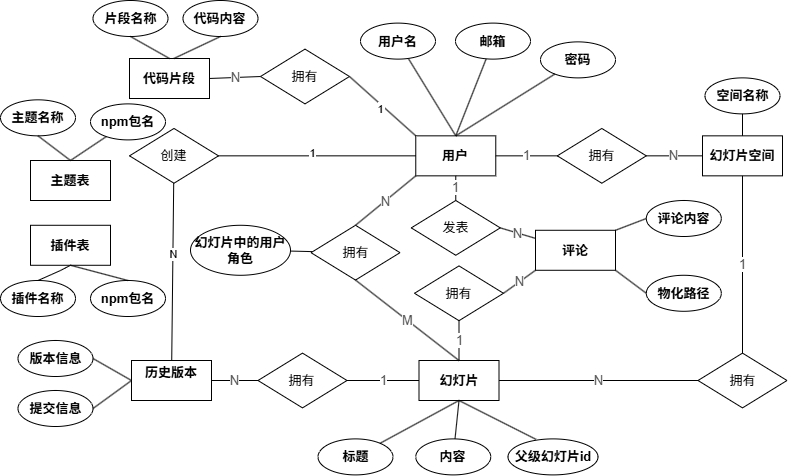
\includegraphics[width=0.9\textwidth]{figures/drawio/核心实体关系图-v4-without-register-code.drawio.png}
        \caption{数据库E-R图}
        \label{fig:er-diagram}
    \end{figure}
    % 主要关系包括：
    % 用户与空间：一个用户可以拥有多个幻灯片空间（一对多关系）；
    % 空间与幻灯片：一个空间可以包含多个幻灯片（一对多关系）；
    % 幻灯片与版本：一个幻灯片可以有多个版本（一对多关系）；
    % 用户与权限：一个用户可以在多个幻灯片中拥有不同的权限（多对多关系）；
    % 幻灯片与评论：一个幻灯片可以有多个评论（一对多关系）。
    \subsection{数据表设计}

    \begin{enumerate}

    \item users 用户表

    用户表存储账户信息，包括用户名、密码哈希值、头像URL等字段，
    用户上传的头像图片将存储至OSS（Object Storage Service，对象存储服务），将返回的URL作为用户头像信息。
    % 同时，每个用户的注册都需要注册码，通过使用registration\_code\_id来记录。
    用户表结构如表\ref{tab:users}所示。

    \begin{table}[htbp]
        \centering
        \caption{users 用户表结构}
        \label{tab:users}
        \begin{tabular}{llll}
            \toprule
            字段名                    & 数据类型         & 是否允许空 & 说明        \\
            \midrule
            id                     & bigint       & 否     & 用户唯一主键    \\
            username               & varchar(50)  & 否     & 用户名       \\
            email                  & varchar(100) & 否     & 邮箱地址      \\
            password\_hash         & varchar(255) & 否     & 密码哈希值     \\
            avatar\_url            & varchar(500) & 是     & 头像URL     \\
            % state                  & tinyint      & 否     & 用户状态（1正常） \\
            % registration\_code\_id & bigint       & 是     & 使用的注册码id  \\
            created\_at            & datetime     & 否     & 创建时间      \\
            updated\_at            & datetime     & 否     & 最近更新时间    \\
            \bottomrule
        \end{tabular}
    \end{table}

    \item slide\_spaces 幻灯片空间表

    幻灯片空间表存储幻灯片空间的基本信息，包括空间名称、所有者用户id等字段，
    is\_public仅用于表明幻灯片空间的基本信息是否公开，当它为1时，
    并不代表整个幻灯片空间的所有幻灯片公开，
    幻灯片空间表结构如表\ref{tab:slide-spaces}所示。

    \begin{table}[htbp]
        \centering
        \caption{slide\_spaces 幻灯片空间表结构}
        \label{tab:slide-spaces}
        \begin{tabular}{llll}
            \toprule
            字段名         & 数据类型         & 是否允许空 & 说明            \\
            \midrule
            id          & bigint       & 否     & 空间唯一主键        \\
            name        & varchar(200) & 否     & 空间名称          \\
            owner\_id   & bigint       & 否     & 所有者用户id       \\
            is\_public  & tinyint      & 否     & 是否公开（0私有，1公开） \\
            created\_at & datetime     & 否     & 创建时间          \\
            updated\_at & datetime     & 否     & 最近更新时间        \\
            \bottomrule
        \end{tabular}
    \end{table}
   \item slide\_comments 评论表
   
    评论表评论向相关信息，包括评论正文内容、所属幻灯片id、评论者发表者id、父评论id等字段，
    评论表通过reply\_id和path字段实现评论的树形结构。
    reply\_id指向父评论id，顶层评论的reply\_id为NULL。

    path字段是评论表的物化路径字段，存储从根节点到当前节点的完整路径字符串，如1-5-12。评论一旦发布，它的结构就不会再发生变化。
    当新增一条评论时，只需要把父评论的path加上当前评论的id，就能得到该评论的path。作者可以使用如SELECT * FROM
    slide\_comments WHERE path LIKE '1-5-\%'的SQL查询语句，一次性获取任意评论节点下的所有子孙评论，不需要递归查询；
    删除某条评论及其所有回复时同样也只需要一条如DELETE FROM slide\_comments WHERE path LIKE
    '1-5-\%'的SQL语句，不需要递归删除。
    评论表结构如表\ref{tab:slide-comments}所示。
    % 另外，评论操作中最频繁的两个场景，正好是物化路径比较擅长的：
    % 一个是展开某条评论下的所有回复，这时候只需要执行如SELECT * FROM slide\_comments WHERE path LIKE '1-5-\%'这样一条SQL查询，
    % 就可以一次性把整个子树取出来，不用递归；另一个是删除某条评论以及它下面的所有子孙回复，
    % 同样可以通过类似 DELETE FROM slide\_comments WHERE path LIKE '1-5-\%' 的单条语句搞定，
    % 这样就避免了逐节点递归删除带来的多次数据库往返。物化路径用冗余一个 path 字段作为代价，
    % 把子树查询和删除的复杂度从递归所需的 $O(n)$ 次查询降到了常数次。在评论这种结构固定、子树操作又比较频繁的场景下，这个做法的性价比确实很高。


    \begin{table}[htbp]
        \centering
        \caption{slide\_comments 评论表结构}
        \label{tab:slide-comments}
        \begin{tabular}{llll}
            \toprule
            字段名         & 数据类型          & 是否允许空 & 说明              \\
            \midrule
            id          & bigint        & 否     & 评论唯一主键          \\
            slide\_id   & bigint        & 否     & 所属幻灯片id         \\
            user\_id    & bigint        & 否     & 评论发表者id         \\
            content     & text          & 否     & 评论正文内容          \\
            path        & varchar(1000) & 否     & 根节点到本节点的物化路径    \\
            reply\_id   & bigint        & 是     & 父评论id，顶层评论为NULL \\
            created\_at & datetime      & 否     & 评论发布时间          \\
            \bottomrule
        \end{tabular}
    \end{table}
    \item slides 幻灯片表

    幻灯片表存储每个幻灯片文档相关信息，包括幻灯片Markdown源码、所属空间id、预览URL  等字段。
    preview\_url是Slidev构建好的幻灯片预览图片，方便用户在幻灯片列表中快速浏览幻灯片内容。
    is\_public字段用于说明幻灯片是否公开，未公开时，只有具有查阅权限的协作者才能访问该链接。
    created\_by作为冗余字段（其值等于slide\_spaces表的owner\_id），可在部分查询中减少内联接。
    parent\_id字段自关联到同表id，实现任意深度的树形结构，根节点的parent\_id为NULL。
    本平台支持用户拖拽来调整目录树的结构，此时，目录树结构可能会经常变动。
    如果引入物化路径，那么用户每次移动一个节点，都需要更新该节点及其所有子孙节点的path字段，这样会大大增加计算复杂度。
    因此，文档树这边只维护parent\_id字段，移动节点的时候只需要修改该记录的父节点引用。
    删除文档节点时则通过BFS(Breadth First Search)遍历查找所有要删除的节点，然后一并删除。
    幻灯片表结构如表\ref{tab:slides}所示。  
    \begin{table}[htbp]
        \centering
        \caption{slides 幻灯片表结构}
        \label{tab:slides}
        \begin{tabular}{llll}
            \toprule
            字段名              & 数据类型         & 是否允许空 & 说明              \\
            \midrule
            id               & bigint       & 否     & 文档唯一主键          \\
            title            & varchar(200) & 否     & 文档标题            \\
            content          & longtext     & 是     & 幻灯片Markdown源码   \\
            slide\_space\_id & bigint       & 否     & 所属空间id          \\
            parent\_id       & bigint       & 是     & 父文档id，根节点为NULL  \\
            allow\_comment   & tinyint      & 否     & 是否允许评论（1允许，0禁止） \\
            created\_by      & bigint       & 否     & 创建者用户id         \\
            is\_public       & tinyint      & 否     & 是否公开（0私有，1公开）   \\
            is\_build        & tinyint      & 否     & 是否已构建为静态页面       \\
            preview\_url     & varchar(255) & 是     & 预览图片URL         \\
            created\_at      & datetime     & 否     & 创建时间            \\
            updated\_at      & datetime     & 否     & 最近修改时间          \\
            \bottomrule
        \end{tabular}
    \end{table}

    \item slide\_versions 历史版本表

    历史版本表记录幻灯片的版本历史，
    % 包括版本内容快照、提交说明、创建者用户id等字段。
    包括版本内容快照、提交说明、创建者用户id等字段。
    % 提交说明字段记录的是每次版本提交的摘要信息，
    % 每个版本的幻灯片源码都会完整存为一条记录，
    创建者用户id不仅可以是幻灯片文档的所有者id，
    也可以是具有编辑权限的协作者的id，
    历史版本表结构如表\ref{tab:slide-versions}所示。

    \begin{table}[htbp]
        \centering
        \caption{slide\_versions 历史版本表结构}
        \label{tab:slide-versions}
        \begin{tabular}{llll}
            \toprule
            字段名         & 数据类型         & 是否允许空 & 说明      \\
            \midrule
            id          & bigint       & 否     & 版本唯一主键  \\
            slide\_id   & bigint       & 否     & 所属幻灯片id \\
            content     & longtext     & 是     & 版本内容快照  \\
            commit\_msg & varchar(500) & 是     & 提交说明    \\
            created\_by & bigint       & 否     & 创建者用户id \\
            created\_at & datetime     & 否     & 创建时间    \\
            \bottomrule
        \end{tabular}
    \end{table}

    \item slide\_user\_roles 用户角色表

    用户角色表定义用户在幻灯片中的角色，
    主要包括幻灯片id、用户id、角色等字段，
    角色字段为enum，可以为owner、editor、commenter、viewer之一，
    用于控制幻灯片协作者的权限。
    用户角色表结构如表\ref{tab:slide-user-roles}所示。

    \begin{table}[htbp]
        \centering
        \caption{slide\_user\_roles 用户角色表结构}
        \label{tab:slide-user-roles}
        \begin{tabular}{llll}
            \toprule
            字段名         & 数据类型     & 是否允许空 & 说明                                \\
            \midrule
            id          & bigint   & 否     & 角色记录主键                            \\
            slide\_id   & bigint   & 否     & 幻灯片id                             \\
            user\_id    & bigint   & 否     & 用户id                              \\
            role        & enum     & 否     & 角色（owner/editor/commenter/viewer） \\
            created\_at & datetime & 否     & 创建时间                              \\
            \bottomrule
        \end{tabular}
    \end{table}

 

    \item snippets 代码片段表

    代码片段表用于存储用户创建的自定义代码片段，包括所属用户id、片段名称、片段内容、创建时间等字段，
    片段名称不仅帮助用户区分不同的代码片段，还可以作为编辑器代码提示的检索关键词，
    用户在编辑幻灯片时，编辑器会根据片段名称前缀检索显示需要插入的代码片段。
    代码片段表结构如表\ref{tab:snippets}所示。
    % 避免重复编写相似代码，提升工作效率。
    % 代码片段表用于存储用户创建的代码块，支持跨文档快速复用。每个代码片段关联到特定用户，
    % 用户可在编辑幻灯片时检索并插入已保存的片段，避免重复编写相似代码，提升工作效率。

    \begin{table}[htbp]
        \centering
        \caption{snippets 代码片段表结构}
        \label{tab:snippets}
        \begin{tabular}{llll}
            \toprule
            字段名         & 数据类型         & 是否允许空 & 说明     \\
            \midrule
            id          & bigint       & 否     & 片段唯一主键 \\
            user\_id    & bigint       & 否     & 所属用户id \\
            name        & varchar(100) & 否     & 片段名称   \\
            content     & text         & 是     & 片段内容   \\
            created\_at & datetime     & 否     & 创建时间   \\
            updated\_at & datetime     & 否     & 最近更新时间 \\
            \bottomrule
        \end{tabular}
    \end{table}

    % \item registration\_codes 注册码表

    % 注册码表用于管理平台的注册码，
    % 包括注册码字符串 、使用者id、是否已使用、创建时间、过期时间等字段。
    % 因为每个注册码只能使用一次，用户注册时需通过是否已经使用校验注册码的有效性，
    % 同时需要通过过期时间来检验注册码是否过期，
    % 注册码表结构如表\ref{tab:registration-codes}所示。
    % \begin{table}[htbp]
    %     \centering
    %     \caption{registration\_codes 注册码表结构}
    %     \label{tab:registration-codes}
    %     \begin{tabular}{llll}
    %         \toprule
    %         字段名         & 数据类型        & 是否允许空 & 说明             \\
    %         \midrule
    %         id          & bigint      & 否     & 注册码唯一主键        \\
    %         code        & varchar(50) & 否     & 注册码字符串         \\
    %         is\_used    & tinyint     & 否     & 是否已使用（0未用，1已用） \\
    %         used\_by    & bigint      & 是     & 使用者id          \\
    %         used\_at    & datetime    & 是     & 使用时间           \\
    %         % created\_by & bigint      & 是      & 创建者（管理员id）   \\
    %         created\_at & datetime    & 否     & 创建时间           \\ expires\_at & datetime & 是 & 过期时间 \\
    %         \bottomrule
    %     \end{tabular}
    % \end{table}

    \item slidev\_themes 主题表

    Slidev主题表存储平台可用的主题配置，主要包括npm包名、主题名称、主题名称等字段。
    本平台通过npm包名标识每个主题，系统初始化时根据npm包名拉取对应npm包加载到系统，
    % 如slidev-theme-meetup@1.5.3，它的npm包名为slidev-theme-meetup@1.5.3，
    % 主题名称为slidev-theme-meetup，而预览图URL用于显示主题的风格和样式，帮助用户挑选自己喜欢的主题。
    主题表结构如表\ref{tab:slidev-themes}所示。
    \begin{table}[htbp]
        \centering
        \caption{slidev\_themes 主题表结构}
        \label{tab:slidev-themes}
        \begin{tabular}{llll}
            \toprule
            字段名           & 数据类型         & 是否允许空 & 说明     \\
            \midrule
            id            & bigint       & 否     & 主题主键   \\
            package\_name & varchar(200) & 否     & npm包名  \\
            name          & varchar(255) & 否     & 主题名称   \\
            preview\_url  & varchar(500) & 是     & 预览图URL \\
            created\_at   & datetime     & 否     & 创建时间   \\
            updated\_at   & datetime     & 否     & 最近更新时间 \\
            \bottomrule
        \end{tabular}
    \end{table}

    \item slidev\_plugins 插件表

    Slidev插件表存储平台可用的Slidev插件信息，
    主要包括npm包名、插件名称等字段。
    npm包名与插件名称的用途和上文主题表中npm包名与主题名称的用途类似，
    唯一的区别就是没有预览图URL，因为插件作为功能性的拓展，无法通过预览图片详细知道使用效果、如何使用。
    每个插件将package\_name作为唯一标识，用户在排版幻灯片时可选择启用所需插件以增强演示效果，
    % 管理员也可根据需求引入新的社区插件。
    插件表结构如表\ref{tab:slidev-plugins}所示。
    \begin{table}[htbp]
        \centering
        \caption{slidev\_plugins 插件表结构}
        \label{tab:slidev-plugins}
        \begin{tabular}{llll}
            \toprule
            字段名           & 数据类型         & 是否允许空 & 说明     \\
            \midrule
            id            & bigint       & 否     & 插件主键   \\
            package\_name & varchar(200) & 否     & npm包名  \\
            name          & varchar(255) & 否     & 插件名称   \\
            created\_at   & datetime     & 否     & 创建时间   \\
            updated\_at   & datetime     & 否     & 最近更新时间 \\
            \bottomrule
        \end{tabular}
    \end{table}

    % %$1{两表设计思路对比}

    % slides与slide\_comments都采用树形结构来组织数据，不过它们在节点移动和删除上有显而易见的差别。
    % 两者在存储策略上也完全不同，具体对比可见表 \ref{tab:design-contrast}。
    % % slides 与 slide\_comments 均以树形结构组织数据，但两者在节点移动、子树展开和删除三个维度上的使用模式截然不同，由此导致了存储策略的根本差异，具体如表 \ref{tab:design-contrast} 所示。

    % \begin{table}[htbp]
    %     \caption{两表树形存储策略对比}
    %     \label{tab:design-contrast}
    %     \centering
    %     \begin{tabular}{lll}
    %         \toprule
    %         操作维度   & slides（文档树）          & slide\_comments（评论树）      \\
    %         \midrule
    %         节点结构调整 & 需要（支持拖拽排序）           & 不需要（评论发出后不移动）             \\
    %         % 子树展开方式 & 逐级展开（按需加载） & 一次性展开整个讨论串 \\
    %         子树删除方式 & 递归逐节点删除              & 单条 LIKE 前缀匹配删除   \\
    %         树形存储模式 & 仅parent\_id & reply\_id + 物化路径 \\
    %         \bottomrule
    %     \end{tabular}
    % \end{table}

\end{enumerate}

\end{cuzchapter}